\documentclass{beamer}
\usepackage{graphicx}
\usepackage{tikz}
\usetikzlibrary{shapes,arrows}
\usepackage{tikz}
%\usecolortheme{seahorse}
  \setbeamertemplate{footline}[page number]
\usepackage{multirow}
\setbeamertemplate{navigation symbols}{}
\setbeamertemplate{frametitle}[default][center]
\setbeamerfont{frametitle}{shape=\scshape}
\usepackage{color}

\usepackage{csquotes}

\usepackage{xcolor}

\usepackage[flushleft]{threeparttable}

{\title{\textsc{Econ 352 - Measurement} \\ \tiny (See Williamson Ch. 2)}
\author{Trevor S. Gallen}
\date{}
\begin{document}
\renewcommand*{\inserttotalframenumber}{\pageref{lastframe}}


\setbeamertemplate{caption}{\raggedright\insertcaption\par}

\begin{frame}
\titlepage
\end{frame}

\begin{frame}
\frametitle[alignment=center]{What is Macro?}
\begin{itemize}
\item Let's think about how we measure GDP
\bigskip
\item Recall GDP is the dollar value of final output produced during a given period of time within the borders of the United States
\bigskip
\item There are three ways to measure this!
\begin{itemize}
\item Expenditure approach:  cost of all final goods sold
\item Income approach:  all income received by agents contributing to production
\item Value-added approach: sum up all value added 
\end{itemize}
\item Let's dig down in how we measure things!
\end{itemize}
\end{frame}

\begin{frame}
\frametitle[alignment=center]{Coconut Production}
\begin{itemize}
\item Coconut producer owns coconut trees: makes 10 million coconuts sold for \$2 each, earns \$20 million
\bigskip
\item Pays inputs:  \$5 million to workers, \$0.5 million on loan, \$1.5 million to government in taxes
\end{itemize}
\begin{table}
\begin{tabular}{lc}
\hline\hline
\multicolumn{2}{c}{Coconut Producer}\\
\hline
Total Revenue & \$20 million\\
Wages & \$5 million\\
Interest on Loan & \$0.5 million\\
Taxes & \$1.5 million\\
\hline
After-Tax Profits & \$13 million\\
\hline\hline
\end{tabular}
\end{table}
\end{frame}

\begin{frame}
\frametitle[alignment=center]{Coconut Use}
\begin{itemize}
\item 6 million of the 20 million coconuts are used by a restaurant (intermediate good), and 4 million are used by by consumers directly (final good)
\bigskip
\item So need to keep track of restaurant as well!
\bigskip
\item Restaurant sells \$30 million in meals, pays \$12 million for coconuts, pays workers \$4 million in wages and \$3 million in taxes
\end{itemize}
\begin{table}
\begin{tabular}{lcc}
\hline\hline
\multicolumn{2}{c}{Restaurant}\\
\hline
Total Revenue & \$30 million\\
Cost of Coconuts & \$12 million\\
Wages & \$4 million\\
Taxes & \$3 million\\
\hline
After-Tax Profits & \$11 million\\
\hline\hline
\end{tabular}
\end{table}
\end{frame}


\begin{frame}
\frametitle[alignment=center]{Government}
 Government takes in \$5.5 million in taxes (\$1.5 from producer, \$3 from restaurant, and \$1 from consumers) and pays \$5.5. million for soldiers to defend the coconuts
\begin{table}
\begin{tabular}{lcc}
\hline\hline
\multicolumn{2}{c}{Government}\\
\hline
Tax Revenue & \$5.5 million\\
Wages & \$5.5 million\\
\hline\hline
\end{tabular}
\end{table}
\end{frame}


\begin{frame}
\frametitle[alignment=center]{Consumers}
Consumers work for producers, restaurant and govt \$5 mill + \$5.5 mill  + \$4 mill, lend money \$0.5 million, pay taxes \$1 million, and own firms (\$24 million profit)
\begin{table}
\begin{tabular}{lcc}
\hline\hline
\multicolumn{2}{c}{Consumers/Households}\\
\hline
Wage Income & \$14.5 million\\
Interest Income & \$0.5 million\\
Taxes & \$1 million\\
Profits from Producers/Restaurant & \$24 million\\
\hline\hline
\end{tabular}
\end{table}
\end{frame}


\begin{frame}
\frametitle[alignment=center]{Product Approach to Measuring GDP}
\begin{itemize}
\item Let's look at the ``value added" approach:  add up the sum of value added
\item Coconuts sold+restaurant profits after inputs+government expenditure
\item \$20 million for coconuts+ (\$30 million in revenue-\$12 million for coconuts)+\$5.5 million for government
\begin{table}
\begin{tabular}{lcc}
\hline\hline
\multicolumn{2}{c}{Product Approach}\\
\hline
Value added - coconuts & \$20 million\\
Value added - restaurant food & \$18 million\\
Value added - government & \$5.5 million\\
\hline
GDP & \$43.5 million\\
\hline\hline
\end{tabular}
\end{table}
\end{itemize}
\end{frame}

\begin{frame}
\frametitle[alignment=center]{Expenditure Approach to Measuring GDP}
\begin{itemize}
\item $$Y=C+I+G+X$$
\item (\$30 million at restaurants +\$8 million directly)+\$5.5+0
\begin{table}
\begin{tabular}{lcc}
\hline\hline
\multicolumn{2}{c}{Product Approach}\\
\hline
Consumption & \$38 million\\
Investment & \$0 million\\
Government expenditures & \$5.5 million\\
Net exports & \$0 million\\
\hline
GDP & \$43.5 million\\
\hline\hline
\end{tabular}
\end{table}
\end{itemize}
\end{frame}

\begin{frame}
\frametitle[alignment=center]{Clearing up a common misconception}
\begin{itemize}
\item It is sometimes claimed that imports reduce GDP because:
$$Y=C+I+G+Ex-Im$$
Where $Ex$ is exports and $Im$ is imports
\item If I buy an iPhone from China, this is a final good sold in the U.S. and is in $C$. But it wasn't produced in the U.S.!  To avoid double counting, we take it out in $Im$.  
\item The iPhone didn't take away from GDP, it was just completely excluded
\end{itemize}
\end{frame}




\begin{frame}
\frametitle[alignment=center]{Income Approach to Measuring GDP}
\begin{itemize}
\item Wage income+profits+interest income+taxes
\begin{table}
\begin{tabular}{lcc}
\hline\hline
\multicolumn{2}{c}{Product Approach}\\
\hline
Wage income & \$14.5 million\\
After-tax profits & \$24 million\\
Interest income & \$0.5 million\\
Taxes & \$4.5 million\\
\hline
GDP & \$43.5 million\\
\hline\hline
\end{tabular}
\end{table}
\end{itemize}
\end{frame}

\begin{frame}
\frametitle[alignment=center]{Flaws in GDP}
\begin{itemize}
\item What are some flaws in GDP?
\begin{itemize}
\item<2-> Doesn't account for distribution
\bigskip
\item<2-> Leaves out nonmarket activity
\bigskip
\item<2-> Environmental degradation
\bigskip
\item<2-> Government production
\bigskip
\item<2-> Underground economy 
\end{itemize}
\end{itemize}
\end{frame}

\begin{frame}
\frametitle[alignment=center]{Price and Quantity Indicies}
\begin{itemize}
\item We want to compare GDP over time, e.g. if all prices double but quantity stays same, want real GDP not to change!
\bigskip
\item Multiply by constant prices
\end{itemize}
\end{frame}



 \begin{frame}
\frametitle[alignment=center]{Example: Calculating Nominal GDP}
\begin{itemize}
\item Take a set of $N$ goods
$$\text{NomGDP}_t=\sum_{i=1}^NP_{i,t}Q_{i,t}$$
\begin{table}
\centering
\begin{tabular}{lccccccc}
Year & $P_{a,t}$ & $P_{b,t}$ & $Q_{a,t}$ & $Q_{b,t}$ & $GDP_{a,t}$ & $GDP_{b,t}$ & $GDP_t$ \\
\hline
2010 & \$1 & \$1 & 1 & 1 & \$1 & \$1 & \$2 \\
2011 & \$1 & \$2 & 1 & 0.4 & \$1 & \$0.8 & \$1.8 \\
2012 & \$2 & \$1 & 0.8 & 1 & \$1.6 & \$1 & \$2.6 \\
2013 & \$2 & \$2 & 1 & 1 & \$2 & \$2 & \$4 \\
2014 & \$2 & \$2 & 0.5 & 0.5 & \$1 & \$1 & \$2 \\
Eq. & $\cdot$ & $\cdot$ & $\cdot$ & $\cdot$ & $P_{a,t} Q_{a,t}$ & $P_{b,t} Q_{b,t}$ & $GDP_{a,t}$\\
 &  &  &  &  &  &  & $+GDP_{b,t}$
\end{tabular}
\end{table}
\item Why is this troubling?
\begin{itemize}
\item Does $2010\rightarrow 2012$ make sense?
\item Does $2010\rightarrow 2013$ make sense?
\item Does $2010\rightarrow 2014$ make sense?
\end{itemize}
\item How do we fix it?
\end{itemize}
 \end{frame}
 
  \begin{frame}
\frametitle[alignment=center]{Example: Calculating GDP in Constant Dollars-I}
We'll use 2010 prices (denoted by a bar):
$$\text{RealGDP}_t=\sum_{i=1}^N\bar{P_{i}}Q_{i,t}$$
\begin{table}
\centering
\begin{tabular}{lccccccc}
Year & $P_{a,t}$ & $P_{b,t}$ & $Q_{a,t}$ & $Q_{b,t}$ & $GDP_{a,t}$ & $GDP_{b,t}$ & $GDP_t$ \\
\hline
2010 & \$1 & \$1 & 1 & 1 & \$1 & \$1 & \$2 \\
2011 & $\cdot$ & $\cdot$ & 1 & 0.4 & \$1 & \$0.4 & \$1.4 \\
2012 & $\cdot$ & $\cdot$ & 0.8 & 1 & \$0.8 & \$1 & \$1.8\\
2013 & $\cdot$ & $\cdot$ & 1 & 1 & \$1 & \$1 & \$2 \\
2014 & $\cdot$ & $\cdot$ & 0.5 & 0.5 & \$0.5 & \$0.5 & \$1 \\
Eq. & $\cdot$ & $\cdot$ & $\cdot$ & $\cdot$ & ${\color{red}{P_{a,2010}}} Q_{a,t}$ & ${\color{red}{P_{b,2010}}} Q_{b,t}$ & $GDP_{a,t}$\\
 &  &  &  &  &  &  & $+GDP_{b,t}$
\end{tabular}
\end{table}
\normalsize
\begin{itemize}
\item Does $2010\rightarrow 2012$ make sense now?
\item Does $2010\rightarrow 2013$ make sense now?
\item Does $2010\rightarrow 2014$ make sense now?
\end{itemize}
 \end{frame}
 
   \begin{frame}
\frametitle[alignment=center]{Example: Calculating GDP in Constant Dollars-II}
Or use 2014 prices:
\begin{table}
\centering
\begin{tabular}{lccccccc}
Year & $P_{a,t}$ & $P_{b,t}$ & $Q_{a,t}$ & $Q_{b,t}$ & $GDP_{a,t}$ & $GDP_{b,t}$ & $GDP_t$ \\
\hline
2010 & $\cdot$ & $\cdot$ & 1 & 1 & \$2 & \$2 & \$4 \\
2011 & $\cdot$ & $\cdot$ & 1 & 0.4 & \$2 & \$0.8 & \$2.4 \\
2012 & $\cdot$ & $\cdot$ & 0.8 & 1 & \$1.6 & \$2 & \$3.6\\
2013 & $\cdot$ & $\cdot$ & 1 & 1 & \$2 & \$2 & \$4 \\
2014 & $\$2$ & $\$2$ & 0.5 & 0.5 & \$1& \$1 & \$2 \\
Eq. & $\cdot$ & $\cdot$ & $\cdot$ & $\cdot$ & ${\color{red}{P_{a,2014}}} Q_{a,t}$ & ${\color{red}{P_{b,2014}}} Q_{b,t}$ & $GDP_{a,t}$\\
 &  &  &  &  &  &  & $+GDP_{b,t}$
\end{tabular}
\end{table}
\normalsize
\begin{itemize}
\item Does $2010\rightarrow 2012$ make sense now?
\item Does $2010\rightarrow 2013$ make sense now?
\item Does $2010\rightarrow 2014$ make sense now?
\end{itemize}
 \end{frame}
 
    \begin{frame}
\frametitle[alignment=center]{Chain-Weighted GDP}
\begin{itemize}
\item<1-> What's the problem with using ``constant dollars" GDP?
\bigskip
\item<2-> Choice of base year can be incredibly important
\bigskip
\item<3-> We can improve on this with chain-weighted GDP
\bigskip
\begin{enumerate}
\item<4-> Get average price between two years for each good: $\bar{P}_a=\frac{P_{a,t}+P_{a,t+1}}{2},\ \bar{P}_b=\frac{P_{b,t}+P_{b,t+1}}{2}$
\item<5-> Find the new GDP component for each good:  $Q_{a,t}\bar{P}_a+Q_{b,t}\bar{P}_b$ and $Q_{a,t+1}\bar{P}_a+Q_{b,t+1}\bar{P}_b$
\item<6-> Find the percentage difference between the two: $\frac{Q_{a,t+1}\bar{P}_a+Q_{b,t+1}\bar{P}_b}{Q_{a,t}\bar{P}_a+Q_{b,t}\bar{P}_b}$
\item<7-> This gives the ratio of chain-weighted GDP, the growth, but doesn't give us a level
\item<8-> Choose an arbitrary level
\end{enumerate}
\item<9-> Note:  this is slightly simpler than what we actually do.  See online notes for details.
\end{itemize}
 \end{frame}
 
  
    \begin{frame}
\frametitle[alignment=center]{Example: Chain-Weighted GDP}
\small
\begin{table}
\centering
\begin{tabular}{lccccccccc}
Year & $P_{a,t}$ & $P_{b,t}$ & $Q_{a,t}$ & $Q_{b,t}$ & $\frac{GDP_t}{GDP_{t-1}}$ & $GDP_t$\\
\hline
2010 & \$1 & \$1 & 1 & 1 & $\cdot$ & 100\\
2011 & \$1 & \$2 & 1 & 0.4 & 0.64 & 64\\
2012 & \$2 & \$1 & 0.8 & 1  & 1.29 & 82.6\\
2013 & \$2 & \$2 & 1 & 1  & 1.13 & 93.3\\
2014 & \$2 & \$2 & 0.5 & 0.5 & 0.5 & 46\\
\end{tabular}
\end{table}
\begin{itemize}
\item We now have the relative change in GDP between each period.
\item Chain them together and choose an arbitrary starting point 
\end{itemize}
\end{frame}

    \begin{frame}
\frametitle[alignment=center]{Price Level}
\begin{itemize}
\item Real GDP growth tells us how many goods we have (valued at base year)
$$Real GDP Growth=\frac{\sum_{g}^NQ_{g,t}\textcolor{red}{P_{g,base}}}{\sum_{g}^NQ_{g,base}\textcolor{red}{P_{g,base}}}$$
\item Price index tells us how many dollars we need to buy same basket of goods
$$Real Price Level Growth=\frac{\sum_{g}^N\textcolor{red}{Q_{g,base}}P_{g,base}}{\sum_{g}^N\textcolor{red}{Q_{g,base}}P_{g,t}}$$
\item Same idea:  in one you fix prices in the other you fix quantities 
\item Can pick different baskets of $Q$!  What consumers buy (CPI) vs GDP (implicit price deflator)
\end{itemize}
\end{frame}

\begin{frame}
\frametitle[alignment=center]{Nominal and Real GDP over Time}
\begin{figure}
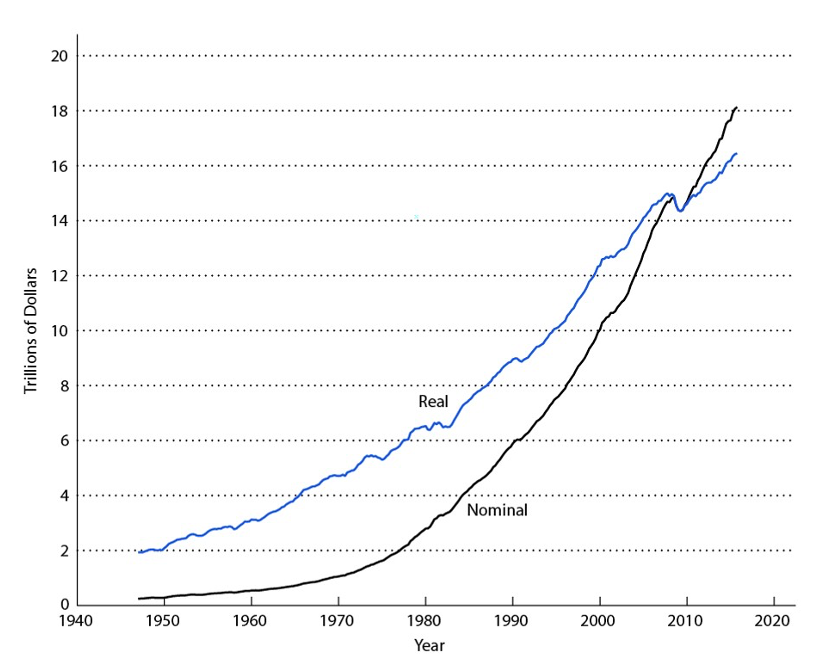
\includegraphics[scale=0.6]{Figures/W_Fig_2pt1.png}
\end{figure}
\end{frame}


\begin{frame}
\frametitle[alignment=center]{CPI Inflation Rate over Time}
\begin{figure}
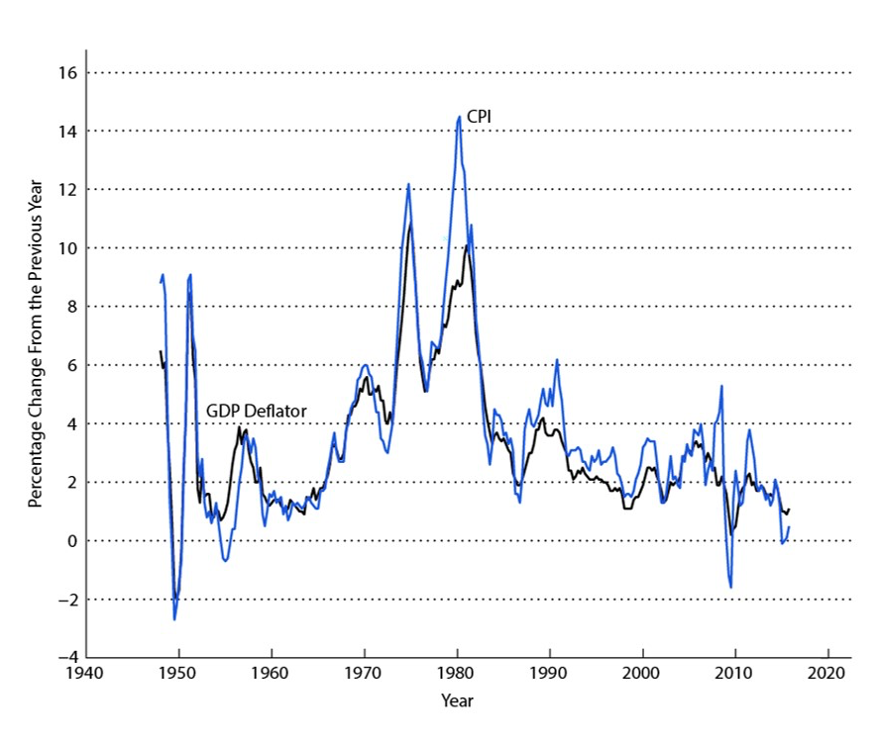
\includegraphics[scale=0.6]{Figures/W_Fig_2pt2.png}
\end{figure}
\end{frame}

\begin{frame}
\frametitle[alignment=center]{CPI vs GDP Deflator}
\begin{figure}
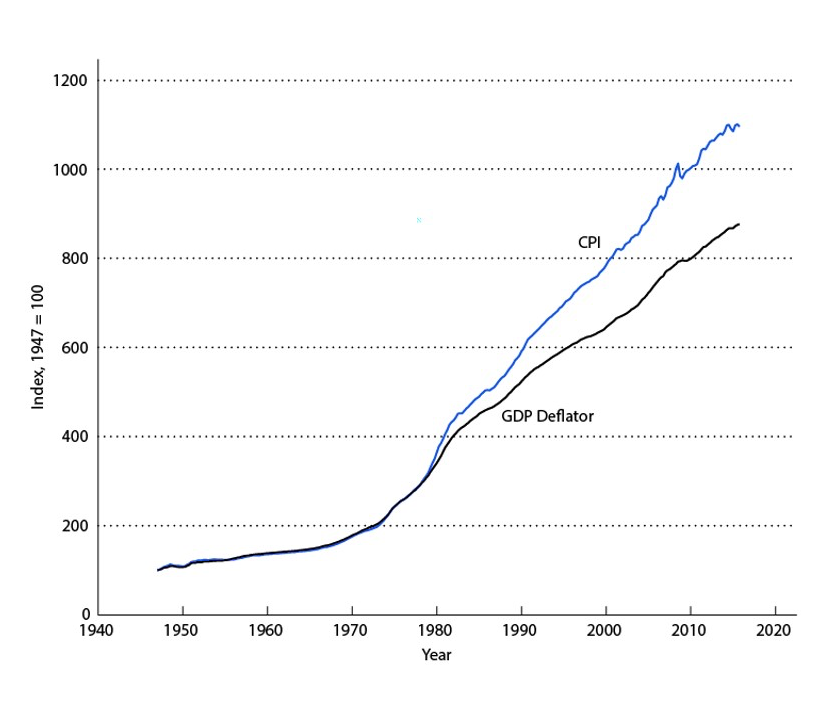
\includegraphics[scale=0.6]{Figures/W_Fig_2pt3.png}
\end{figure}
\end{frame}


\begin{frame}
\frametitle[alignment=center]{Various Inflations}
\begin{figure}
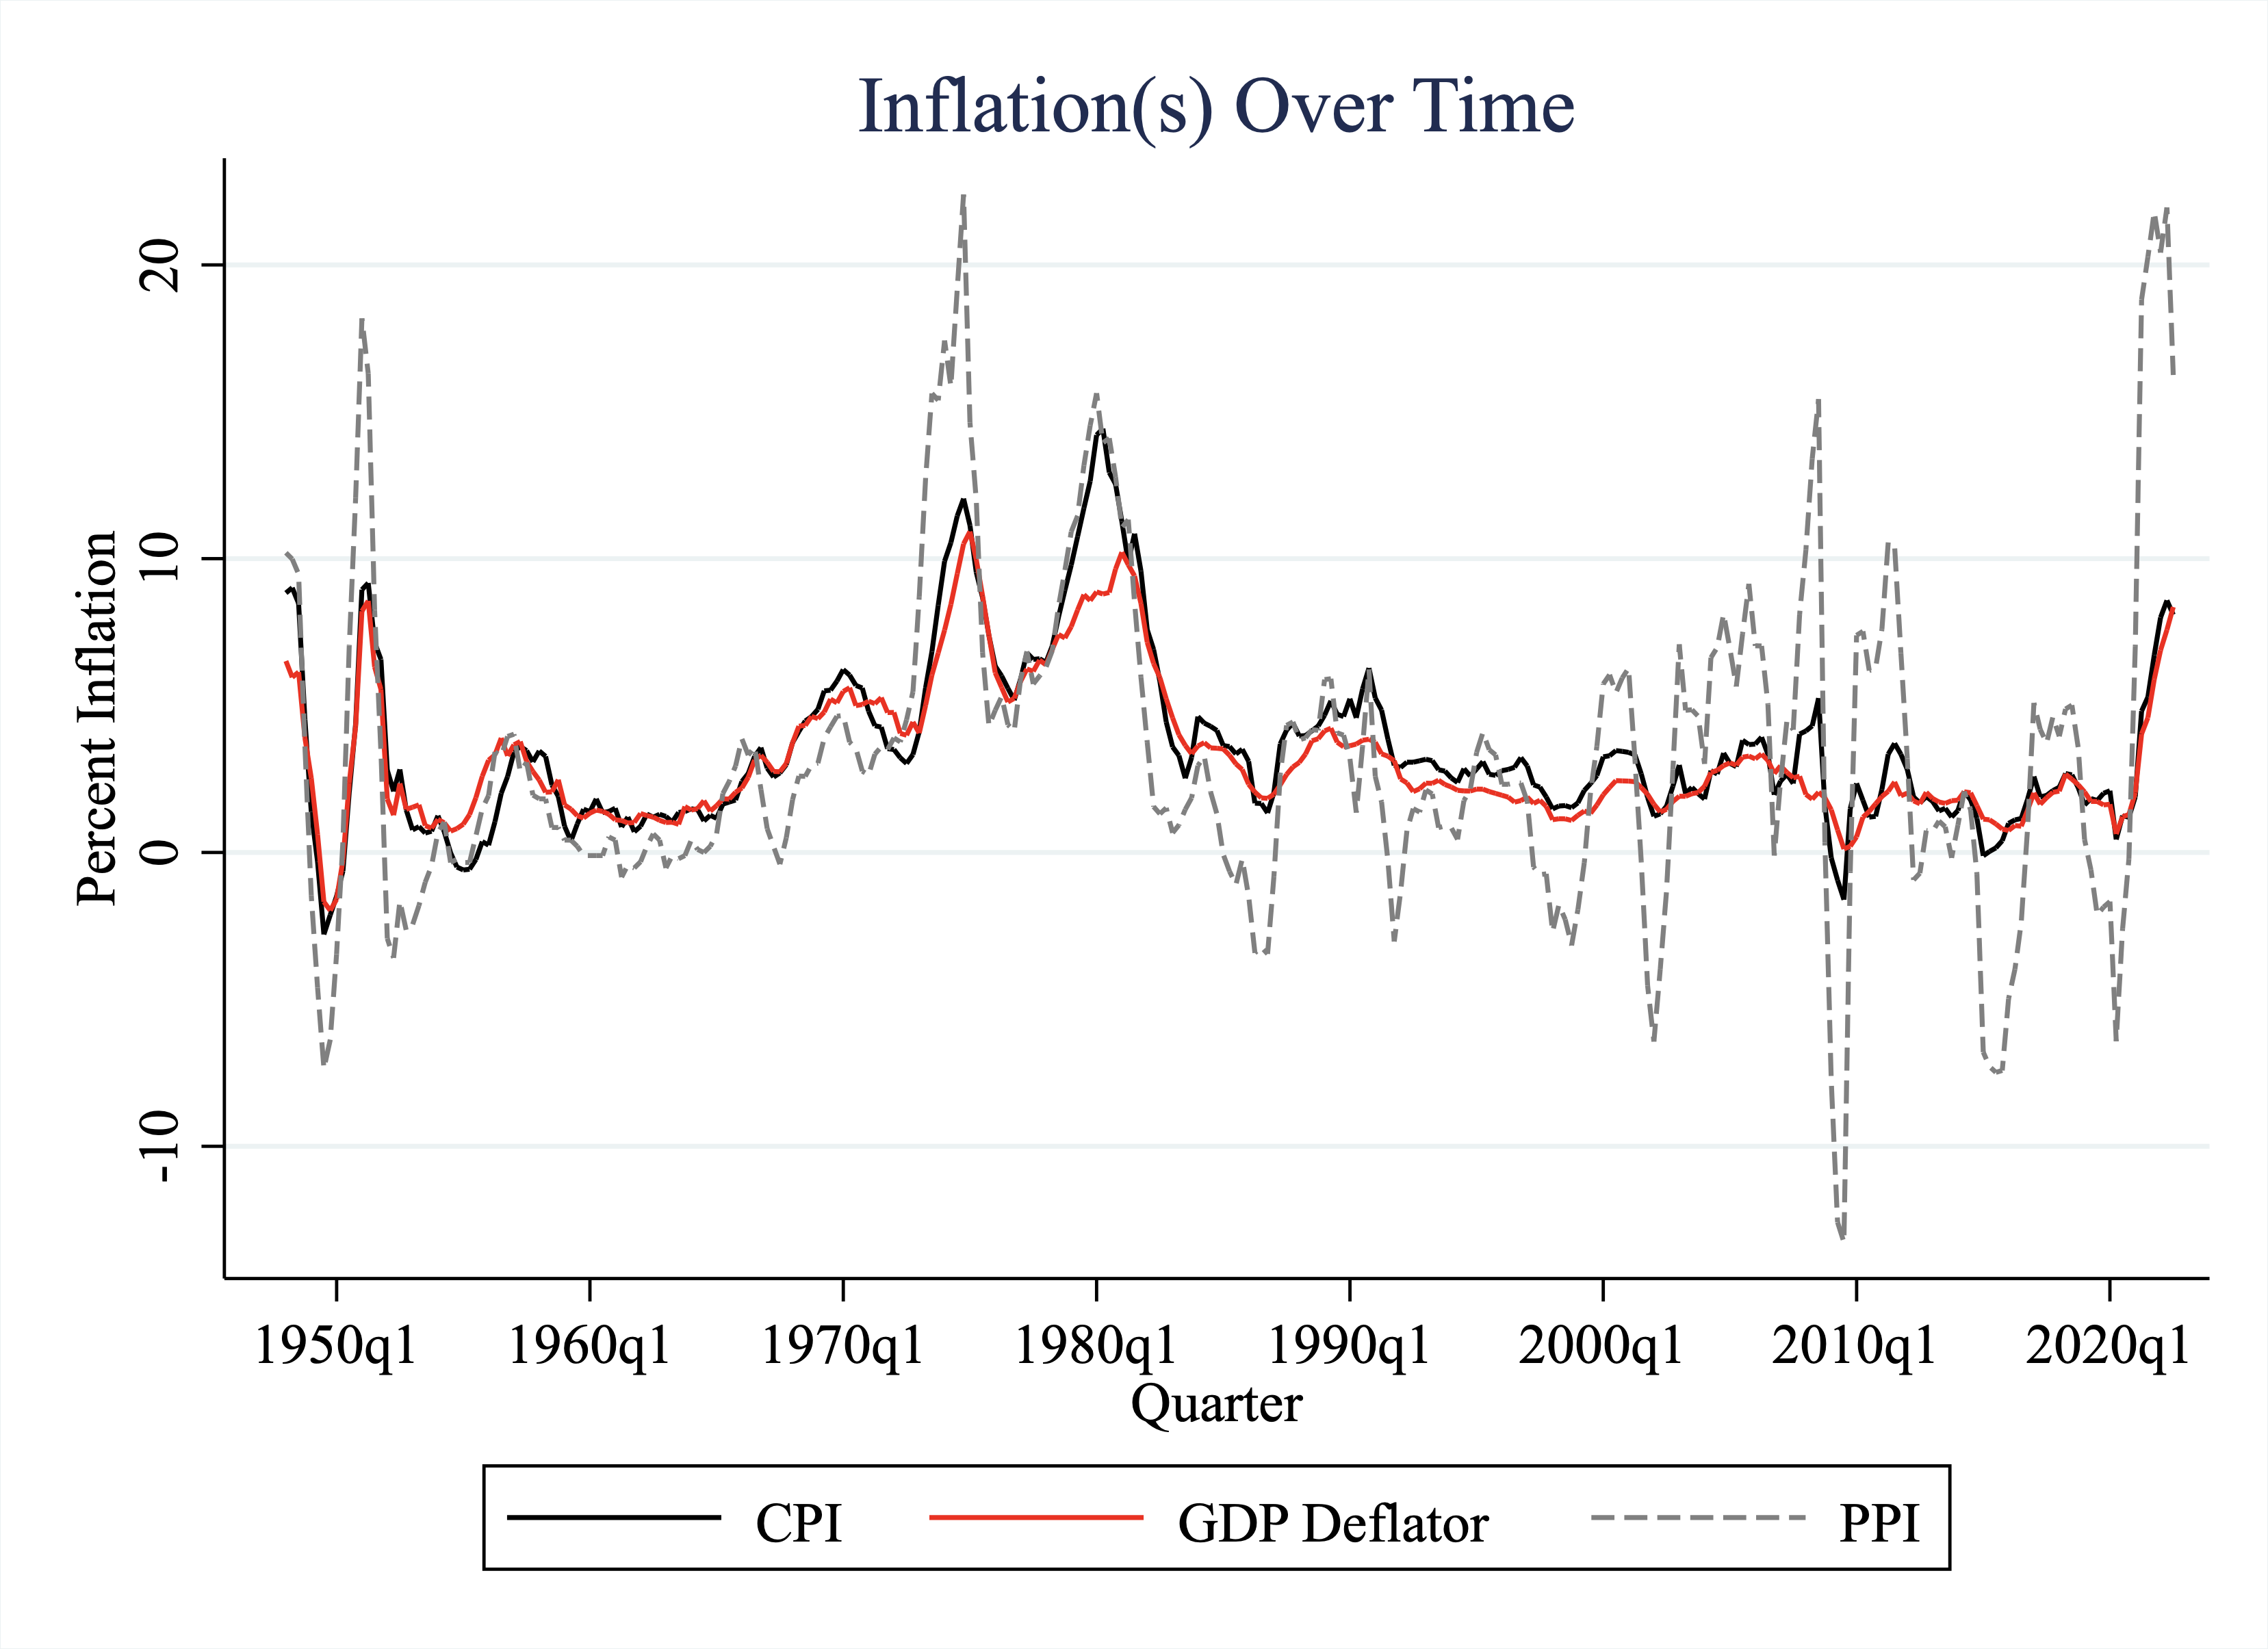
\includegraphics[scale=0.18]{Figures/Fig_CPIs.png}
\end{figure}
\end{frame}


\begin{frame}
\frametitle[alignment=center]{PPI moves more than CPI}
\begin{figure}
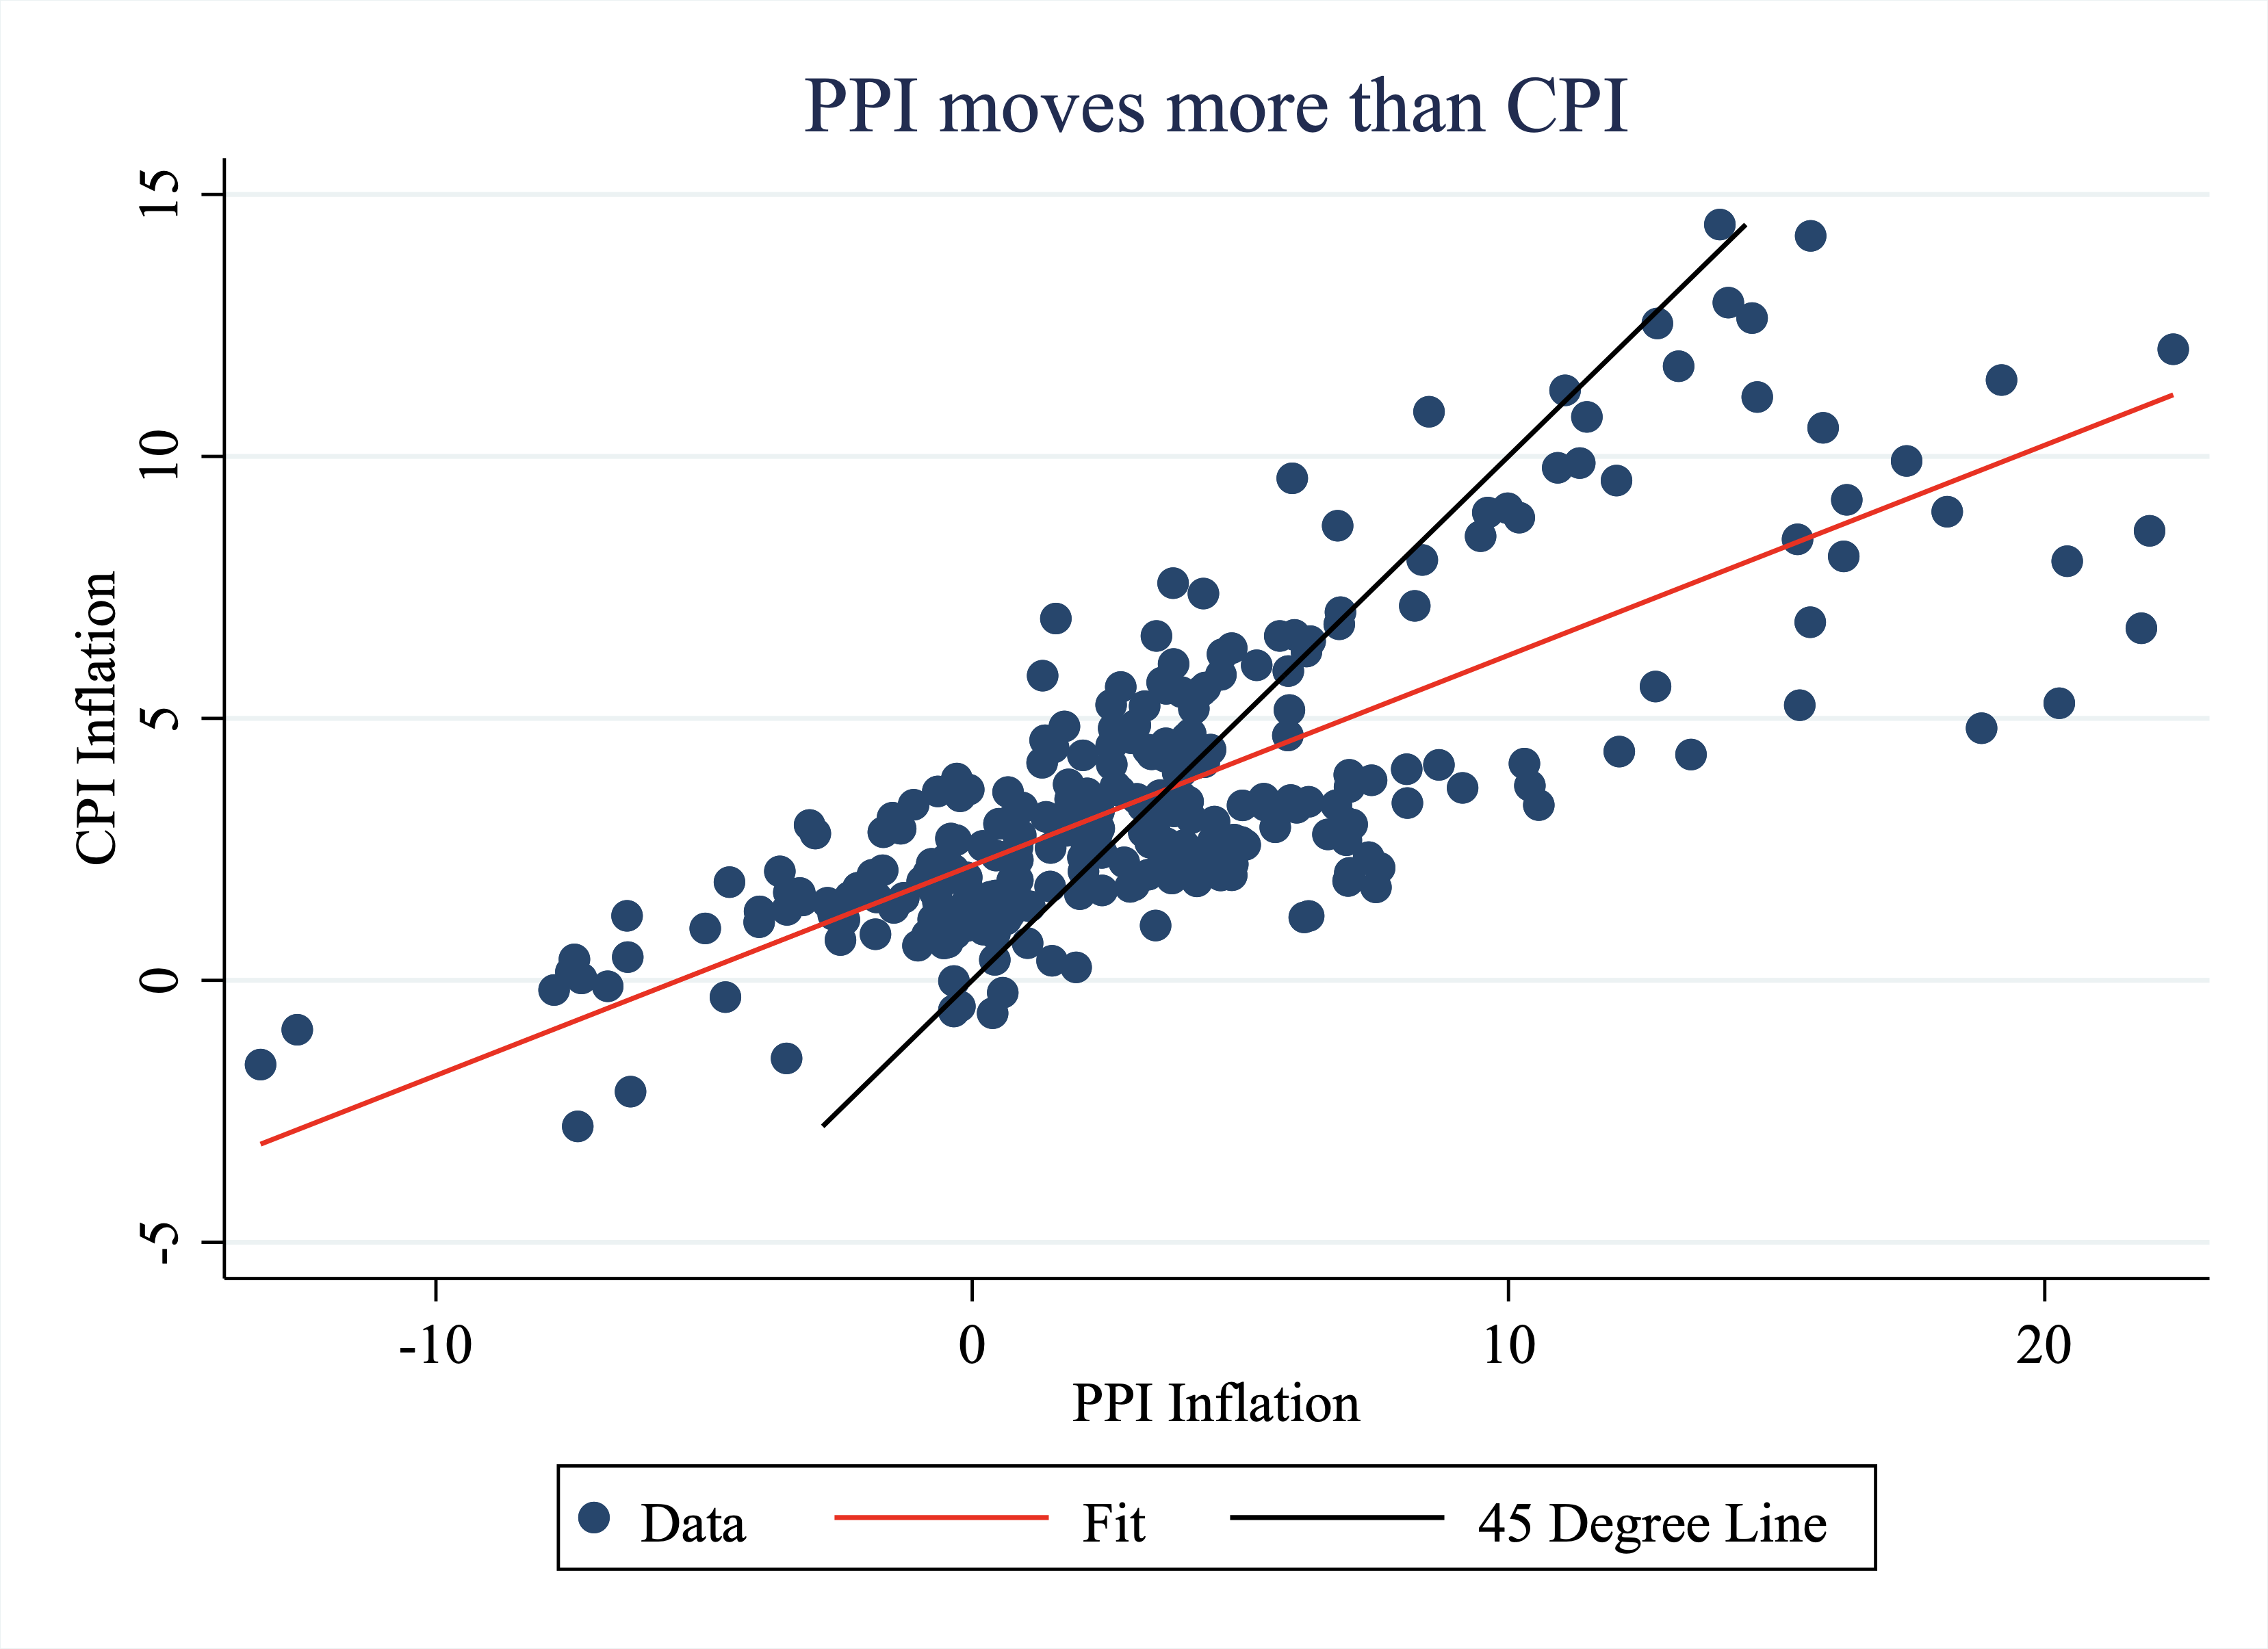
\includegraphics[scale=0.18]{Figures/Fig_CPIvPPI.png}
\end{figure}
\end{frame}


\begin{frame}
\frametitle[alignment=center]{Is this Accurate?}
\begin{figure}

\includegraphics[scale=0.4]{Figures/PPI_Meme.jpeg}
\end{figure}
\end{frame}

    \begin{frame}
\frametitle[alignment=center]{Issues in Measurement}
\begin{itemize}
\item The relative prices of goods change over time: a problem for CPI measurement.
\bigskip
\item The quality of goods and services changes over time.
\bigskip
\item New goods and services are introduced, and some goods and services become obsolete.
\end{itemize}
\end{frame}

    \begin{frame}
\frametitle[alignment=center]{Savings, Wealth, and Capital}
\begin{itemize}
\item The most common issue people have when thinking about GDP is confusing it with wealth
\item GDP is a flow, like income, while wealth is a stock (earned interest would be its income)
\item Similarly, savings (or investment) are flows that contribute to wealth
\item There are many forms savings take, depending on who does it!
\item Private Sector Saving:
$$S^P=Y^D-C=Y+NFP+TR+INT-T-C$$
\item Where:
\begin{itemize}
\item $Y^D$ is disposable income
\item $C$ is consumption
\item $NFP$ is net payments from abroad
\item $TR$ are transfers from govt to households
\item $INT$ is interest paid from govt
\end{itemize}
\item Govt savings is:
$$S^g=T-TR-INT-G$$
\end{itemize}
\end{frame}


    \begin{frame}
\frametitle[alignment=center]{National Savings}
\begin{itemize}
\item In english:  private savings is all production ($Y$) and income from abroad ($NFP$, minus what we eat ($C$), minus the net the government takes away $(TR+INT-T)$
\item In english: government savings is all taxation $T$ minus what it ``eats" ($INT+TR+G$)
\item Note that some private savings is government dissaving.  National saving is:
\begin{align*}S & =S^P+S^g\\
 & =Y+NFP+TR+INT-T-C+T-TR-INT-G\\ 
 & =Y+NFP-C-G
 \end{align*}
\item In english:  What the economy makes $(Y)$, plus what is sent to it $(NFP)$ minus what it ``eats" $(C+G)$
\end{itemize}
\end{frame}

    \begin{frame}
\frametitle[alignment=center]{National Savings}
\begin{itemize}
\item Can use $Y=C+I+G+X$ to get:
$$S=I+NX+NFP$$
\item Where:
\begin{itemize}
\item $I$ is investment
\item $NX$ is net exports
\item $NFP$ is net factor payments from abroad
\end{itemize}
\item $CA=NX+NFP$ is the current account surplus, so:
$$S=I+CA$$
\item In english:  if you produce more than you consume, you either export it, or invest it
\bigskip
\item Alternatively:  you accumulate wealth by creating a capital stock (built by $I$) or having people owe you goods in the future
\end{itemize}
\end{frame}

    \begin{frame}
\frametitle[alignment=center]{Measuring the labor market}
\begin{itemize}
\item We have a few measurements that tell us how the labor market is doing:
$$\text{Labor force}=\text{Number of employed} + \text{number of unemployed}$$
$$\text{Unemployment Rate}=\frac{\text{Number of unemployed}}{\text{Labor force}}$$
$$\text{Participation Rate}=\frac{\text{Labor force}}{\text{Total working age population}}$$
$$\text{Employment/Population Ratio}=\frac{\text{Total Employment}}{\text{Total working age population}}$$
\item Each one measures something different.
\item Unemployment rate:  ``labor market tightness," difficulty in finding a worker for firms, in finding a job for workers
\item Participation rate:  how engaged your overall population is in labor force (how many aren't even looking!)
\item Employment/population ratio:  how much of your potential labor force you're using
%\item My own preference for the last is hours/working age population, which includes the ``intensive" margin of effort
\end{itemize}
\end{frame}

\begin{frame}
\frametitle[alignment=center]{Various Measures of Participation}
\begin{figure}
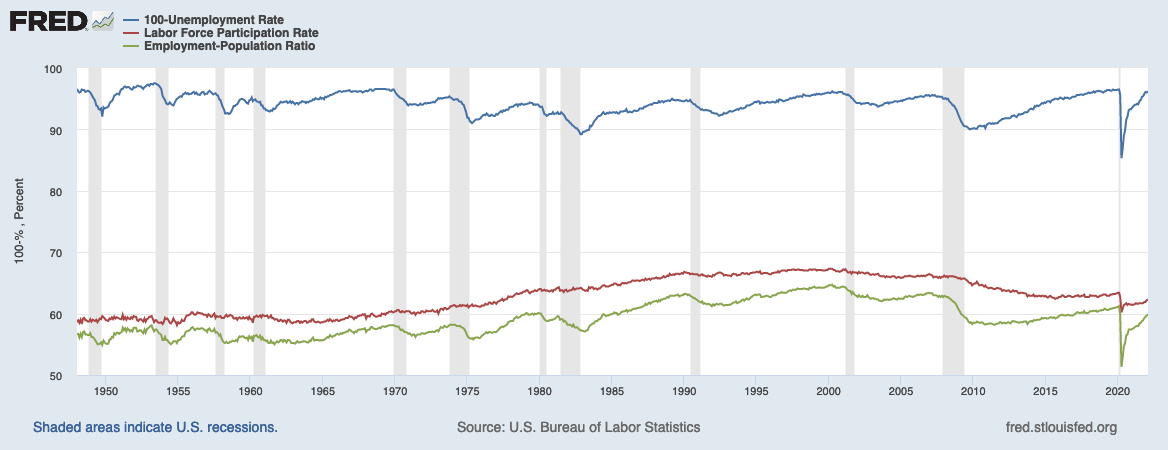
\includegraphics[scale=0.26]{Figures/L2_UI_LFP_EPRatio.png}
\end{figure}
Note I graphed 100-UR
\end{frame}

\begin{frame}
\frametitle[alignment=center]{Unemployment Rate: Alternative Definitions}
\begin{figure}
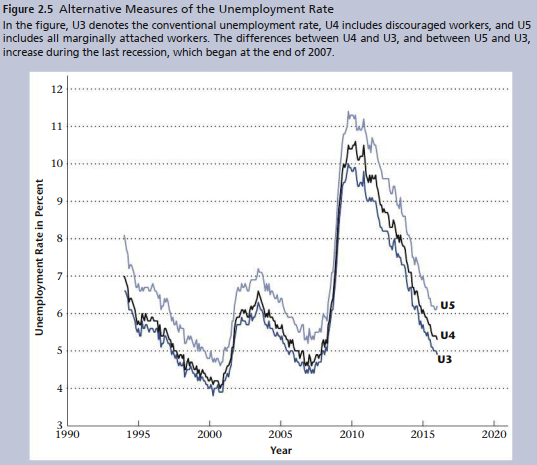
\includegraphics[scale=0.45]{Figures/W_Fig_2pt5.png}
\end{figure}
\end{frame}




\begin{frame}
\frametitle[alignment=center]{Takeaways}
\begin{itemize}
\item Many ways to measure GDP
\bigskip
\item GDP has flaws!
\bigskip
\item We care about real GDP (how calculate)
\bigskip
\item Ways of measuring price index
\bigskip
\item Flows vs stocks: savings
\bigskip
\item  Ways. of measuring the health of the labor market
\end{itemize}
\end{frame}







\end{document}